
I dette projekt er der blevet undersøgt hvordan stormfloden påvirkede fire studieområder i Danmark. De fire områder er Aabenraa, Gedser Havn, Hesnæs og Præstø.\\

Til udvælgningen af studieområderne blev i alt otte kommuner kontaktet. Dette inkluderer Aabenraa, Faaborg-Midtfyn, Guldborgsund, Haderslev, Stevns, Sønderborg og Vordingborg. Udpegningen af potentielle studieområder skete på baggrund af en tabel fra \cite{damberg_vaerste_2023} over højeste målte vandstande i Danmark under 2023-stormfloden. 
Ud af de otte kommuner blev tre kommuner (Aabenraa, Guldborgsund og Vordingborg) udvalgt til videre samarbejde på baggrund af tilgængeligt data. Guldborgsund kommune stillede data fra fire lokaliteter i kommunen til rådighed og der blev udvalgt de to kystbyer, Gedser Havn og Hesnæs, på baggrund af højere målt vandstand under stormfloden.\\

De fire udvalgte studieområder er lokaliseret langs sydkysten af Danmark. På figur \ref{Figur: Oversigtskort} er områdernes placering i Danmark visualiseret.
\begin{figure}[H]
    \centering
    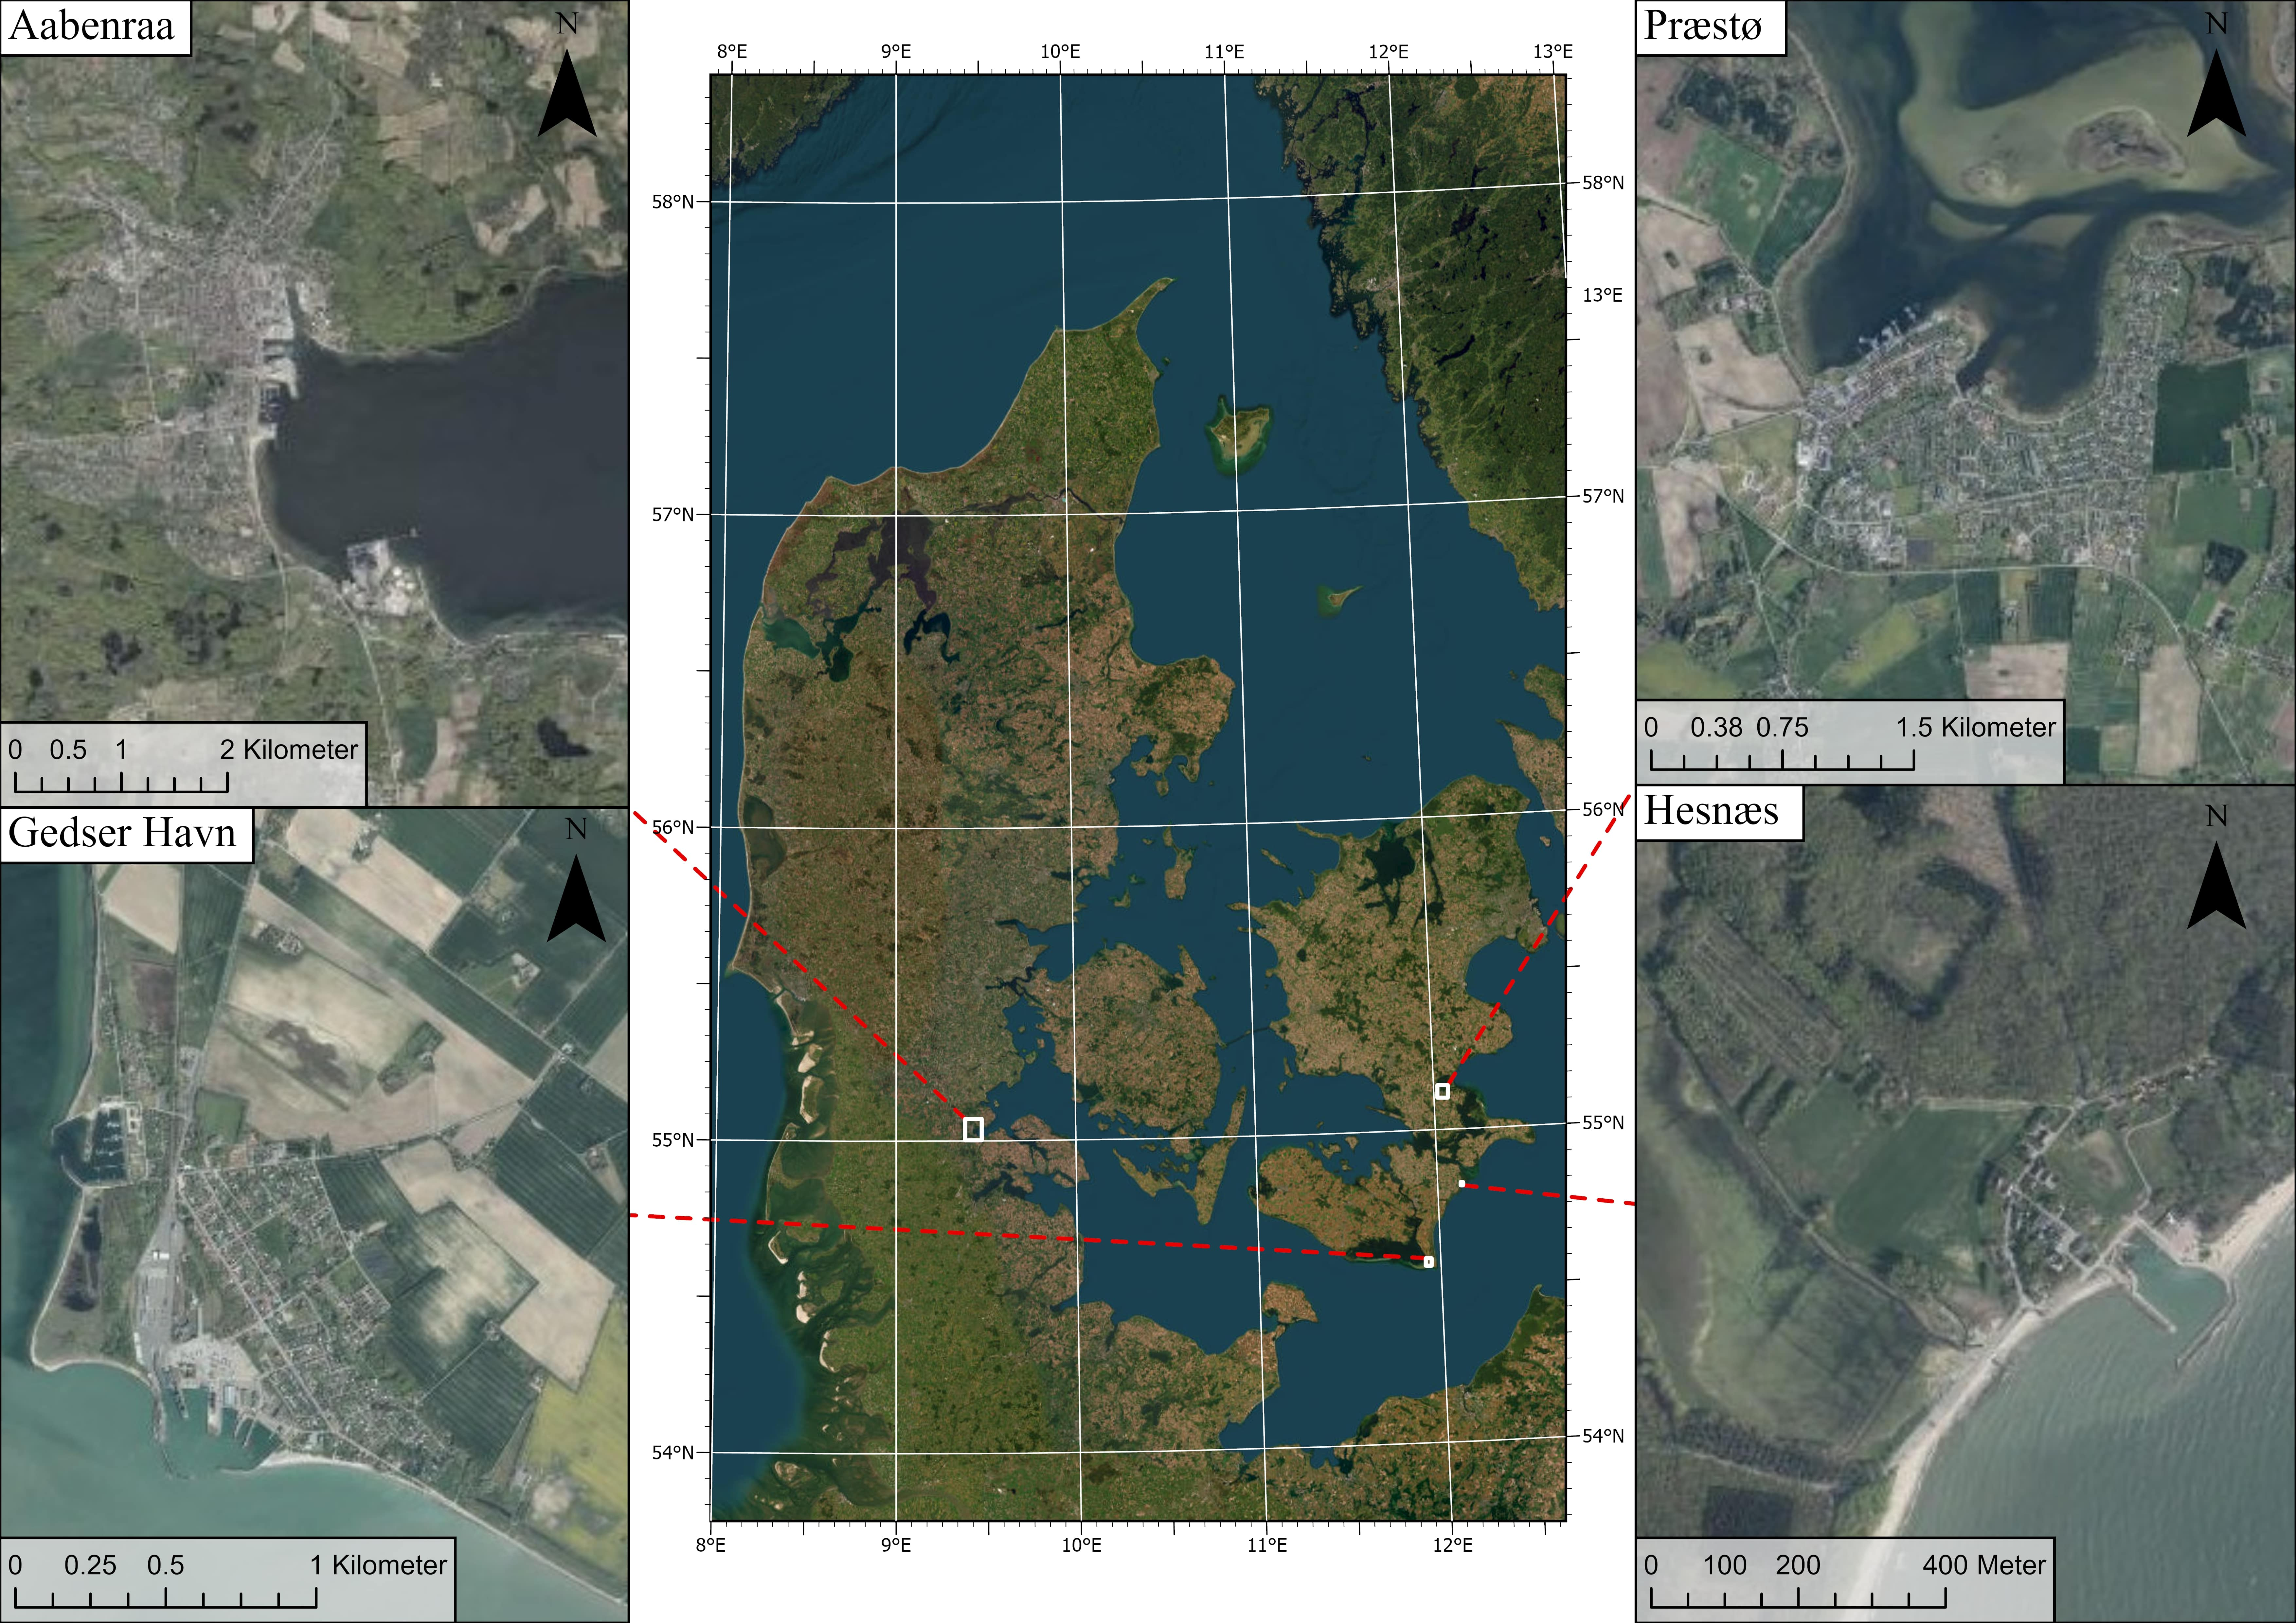
\includegraphics[width=1\linewidth]{images/studieområder/oversigtskort.jpg}
    \caption{Oversigtskort over studieområderne: Aabenraa, Gedser Havn, Hesnæs og Præstø. Baggrundskort fra ESRI og Klimadatastyrelsen.}
    \label{Figur: Oversigtskort}
\end{figure}

{\large Aabenraa}\\
Aabenraa er en by i det sydøstlige Sønderjylland. Byen er beliggende i Aabenraa kommune for enden af den ca. 10 km lange Aabenraa fjord. Byen har en befolkning på 16500 og er den niende største by i Region Syddanmark \citep{danmarks_statistisk_mobile_nodate}. Byen består af to industri havne, Aabenraa og Ensted, og begge er vigtige for skibstrafik med 380 anløbte skibe i 2022 \citep{aabenraa_havn_aabenraa-havn-talogfakta2022_2022}.\\
Aabenraa rapporterede den højeste officielle måling af vandstand under stormfloden på 2,16 meter over DVR90 (figur \ref{Subfig: Aabenraa vandstand}). \\

{\large Gedser Havn}\\
Gedser Havn er en by på sydspidsen af Falster i Guldborgsund kommune. Gedser Havn fungerer som en aktiv fiskerihavn og som en færgehavn til den tyske havn Warnemünde ved Rostock. Byen har et indbyggertal på 670 i 2024 \citep{danmarks_statistisk_mobile_nodate} og er Danmarks sydligste by. \\
Under stormfloden blev der observeret en vandstandsstigning på 1,89 meter over DVR90 i Gedser Havn (figur \ref{Subfig: Gedser vandstand}), den højeste vandstand målt siden 1892, og indstillede færgetrafikken til Tyskland frem til formiddagen den 21. oktober \citep{tiirikainen_sadan_2023}.\\
\begin{figure}[H]
    \begin{subfigure}[b]{0.5\textwidth}
        \centering
        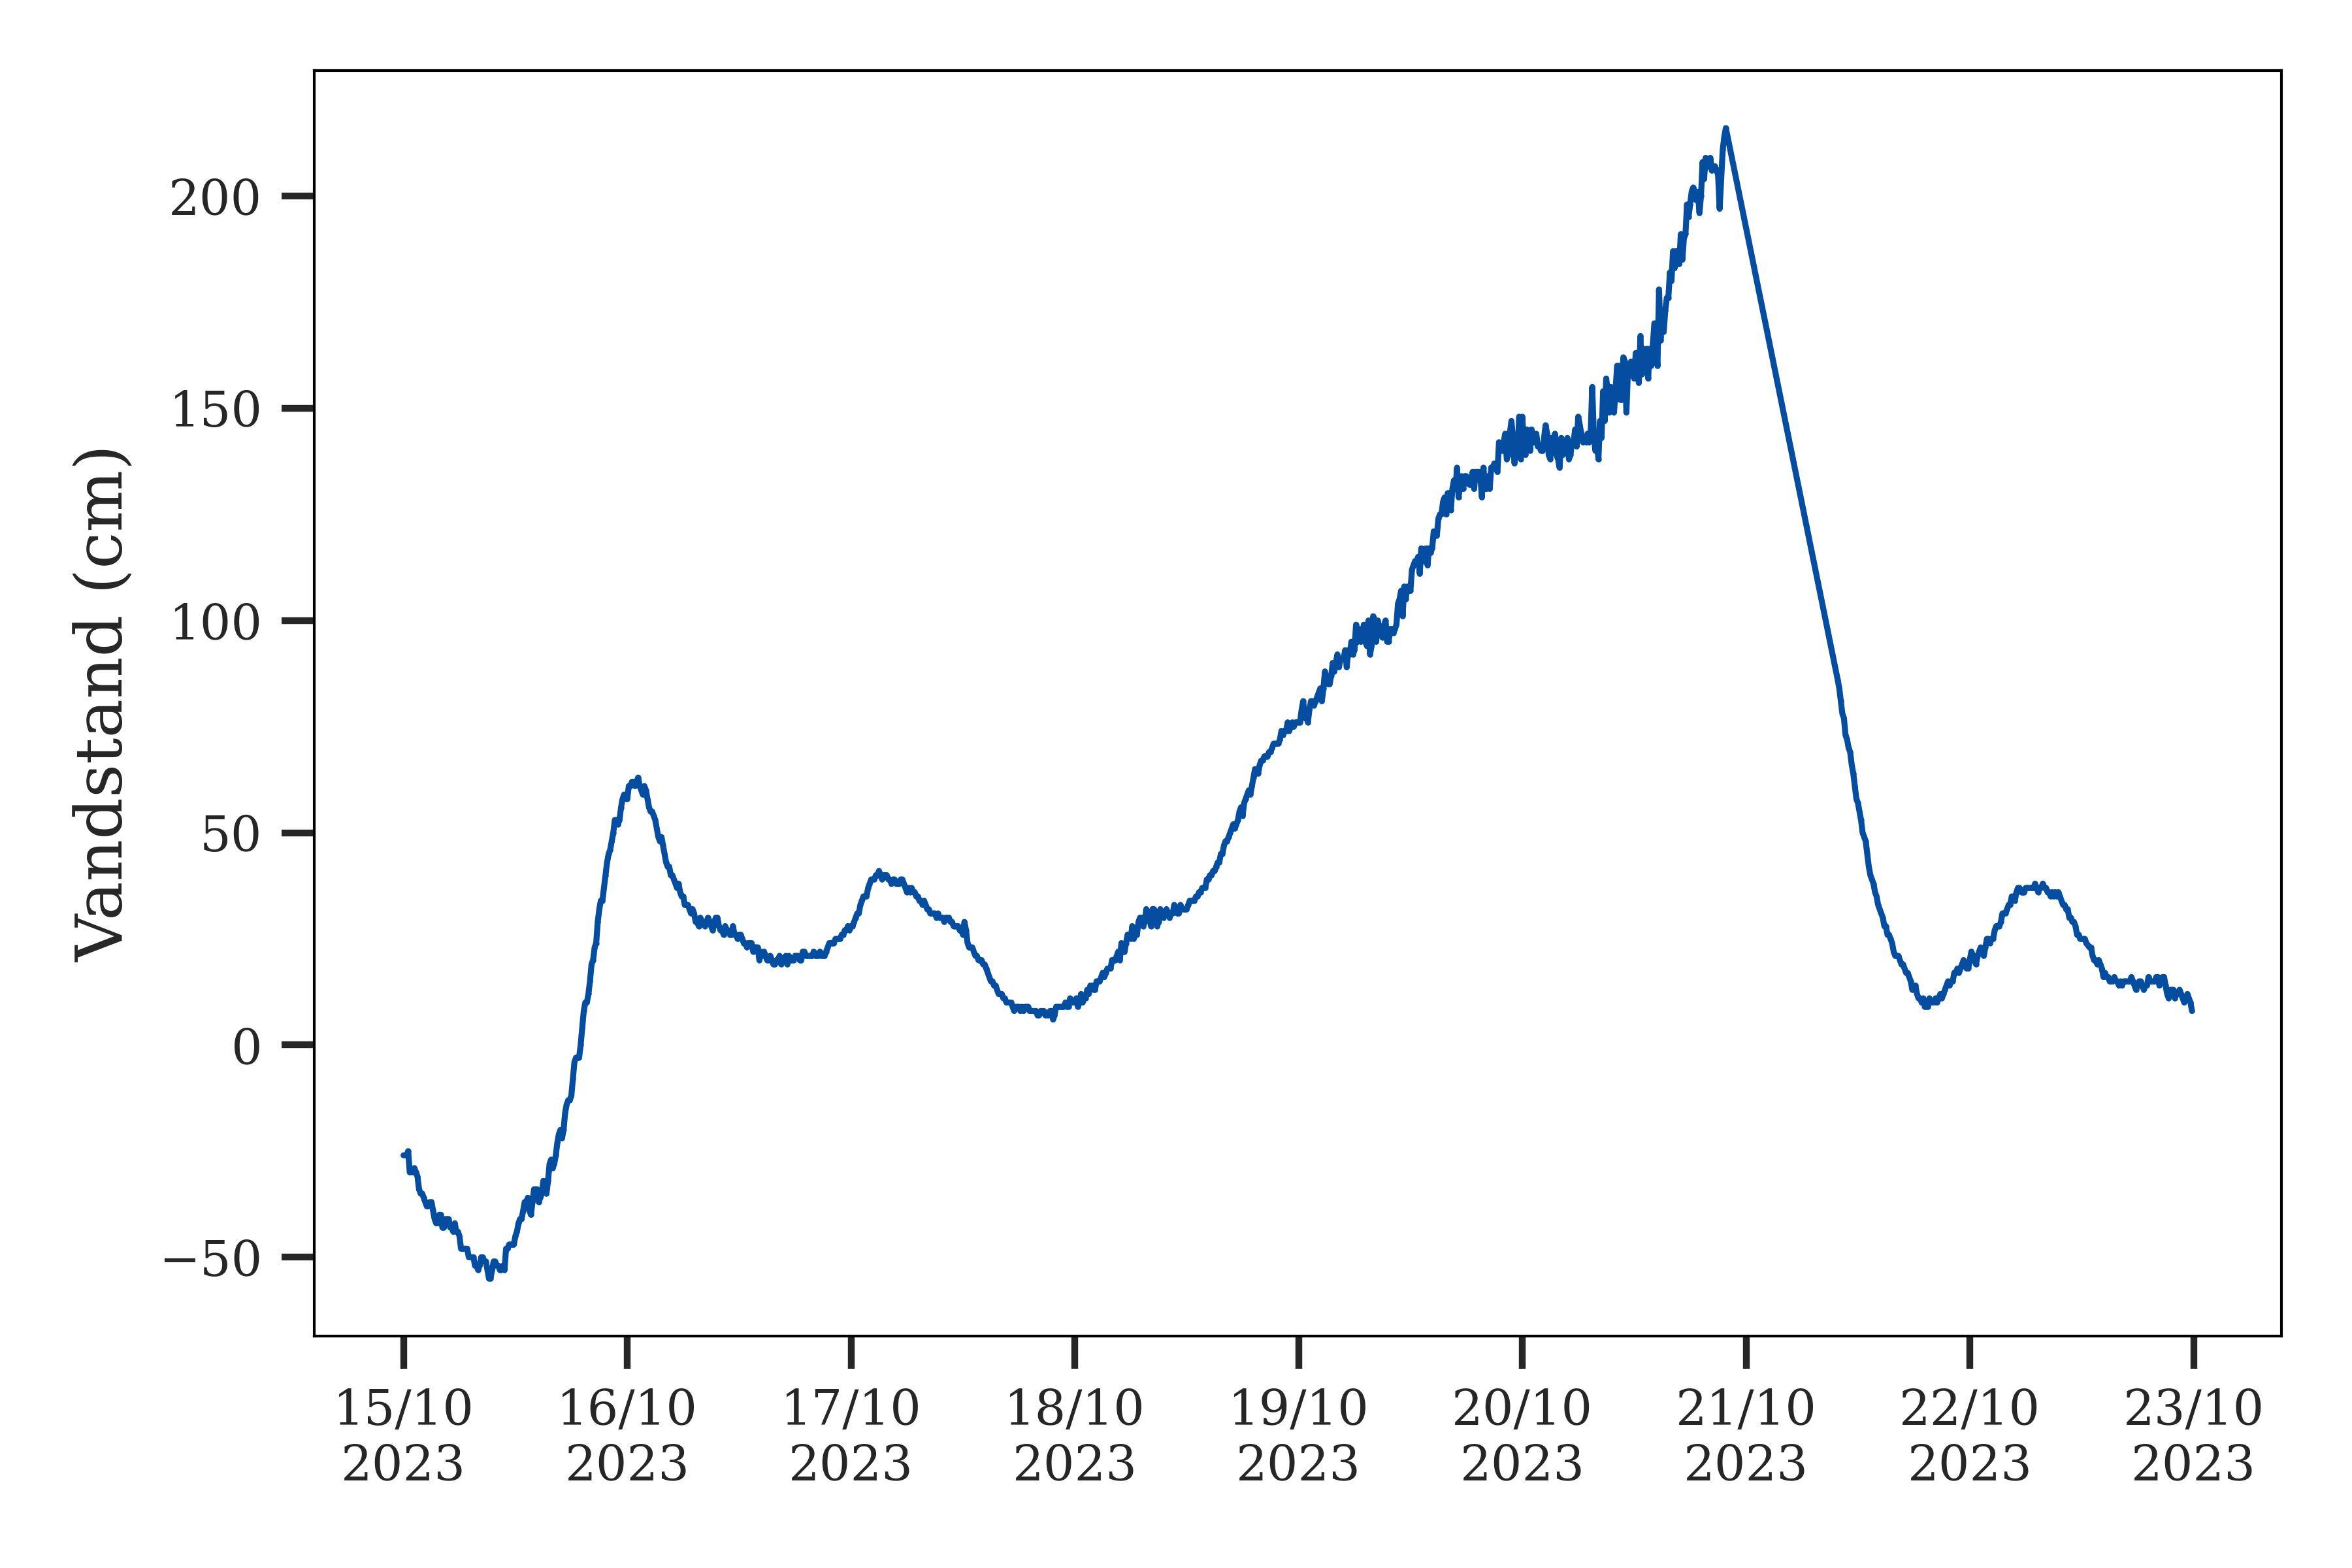
\includegraphics[width=1\textwidth]{images/studieområder/vandstands_grafer/vandstand_aabenraa_vandstandsplot.jpg}
        \caption{}
        \label{Subfig: Aabenraa vandstand}
    \end{subfigure}
    \hspace{0.2cm}
    \begin{subfigure}[b]{0.5\textwidth}
        \centering
        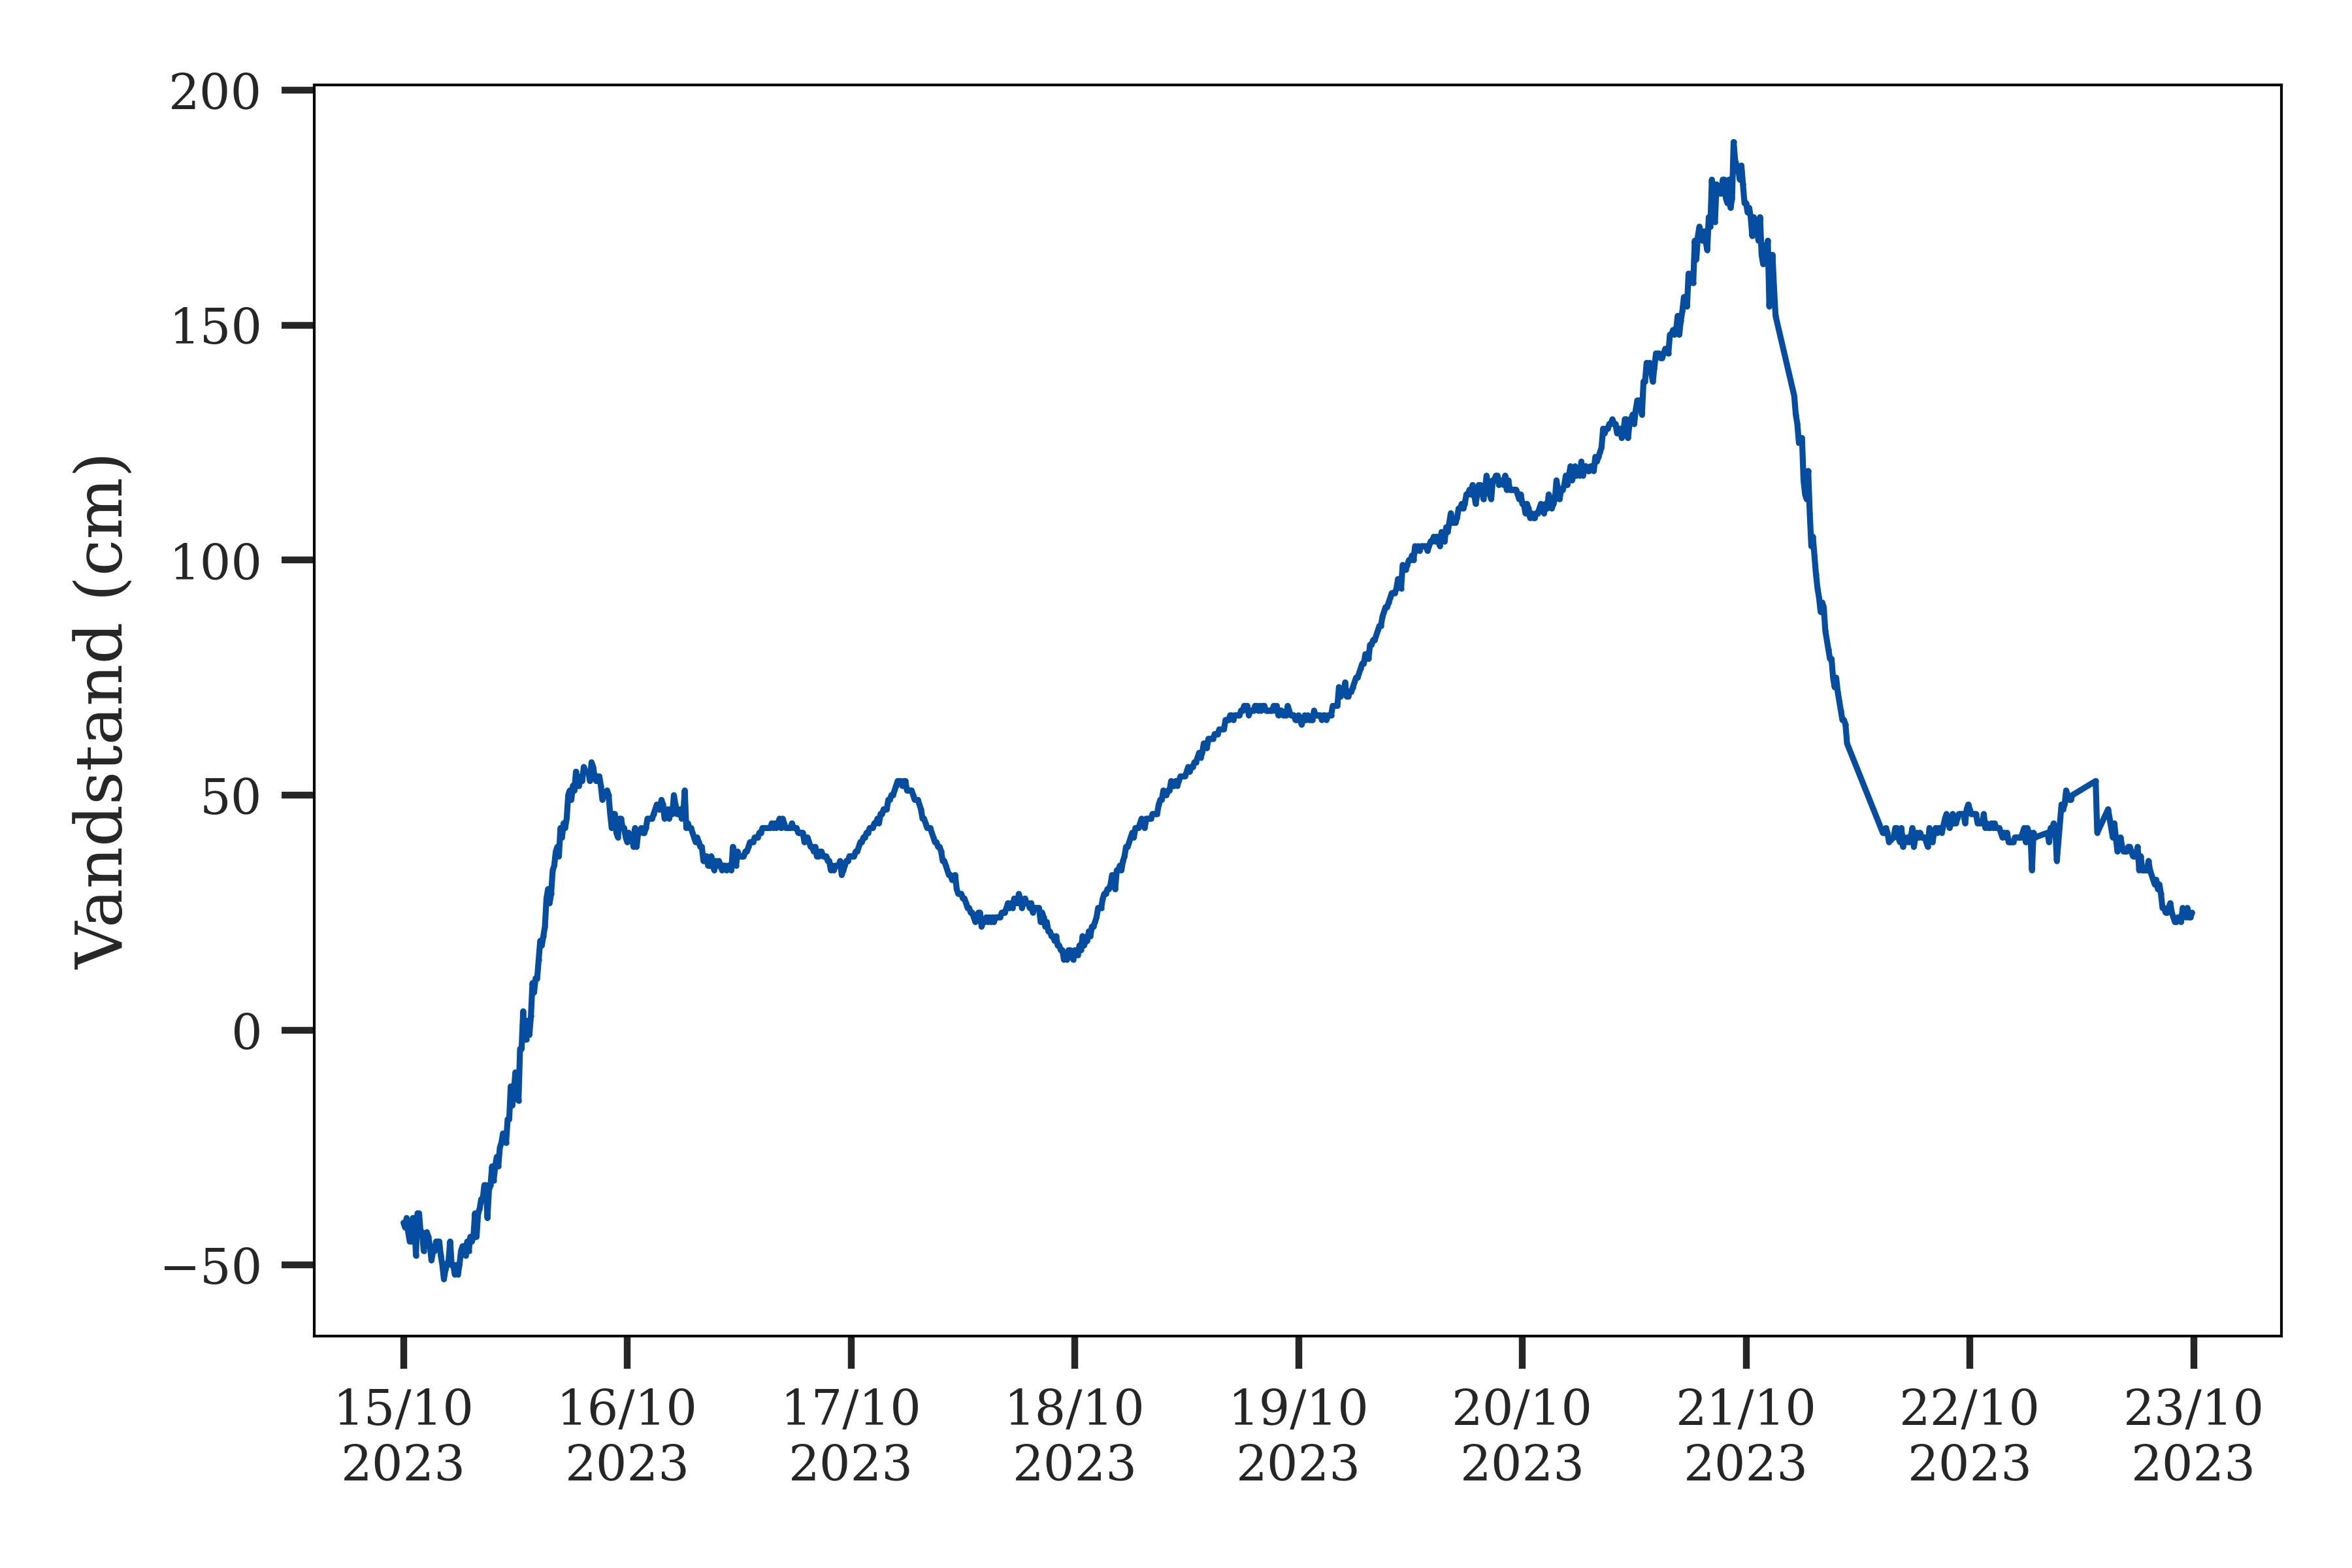
\includegraphics[width=1\textwidth]{images/studieområder/vandstands_grafer/vandstand_gedser_vandstandsplot.jpg}
        \caption{}
        \label{Subfig: Gedser vandstand}
    \end{subfigure}
    \vspace{0.2cm}
    \begin{subfigure}[b]{0.5\textwidth}
        \centering
        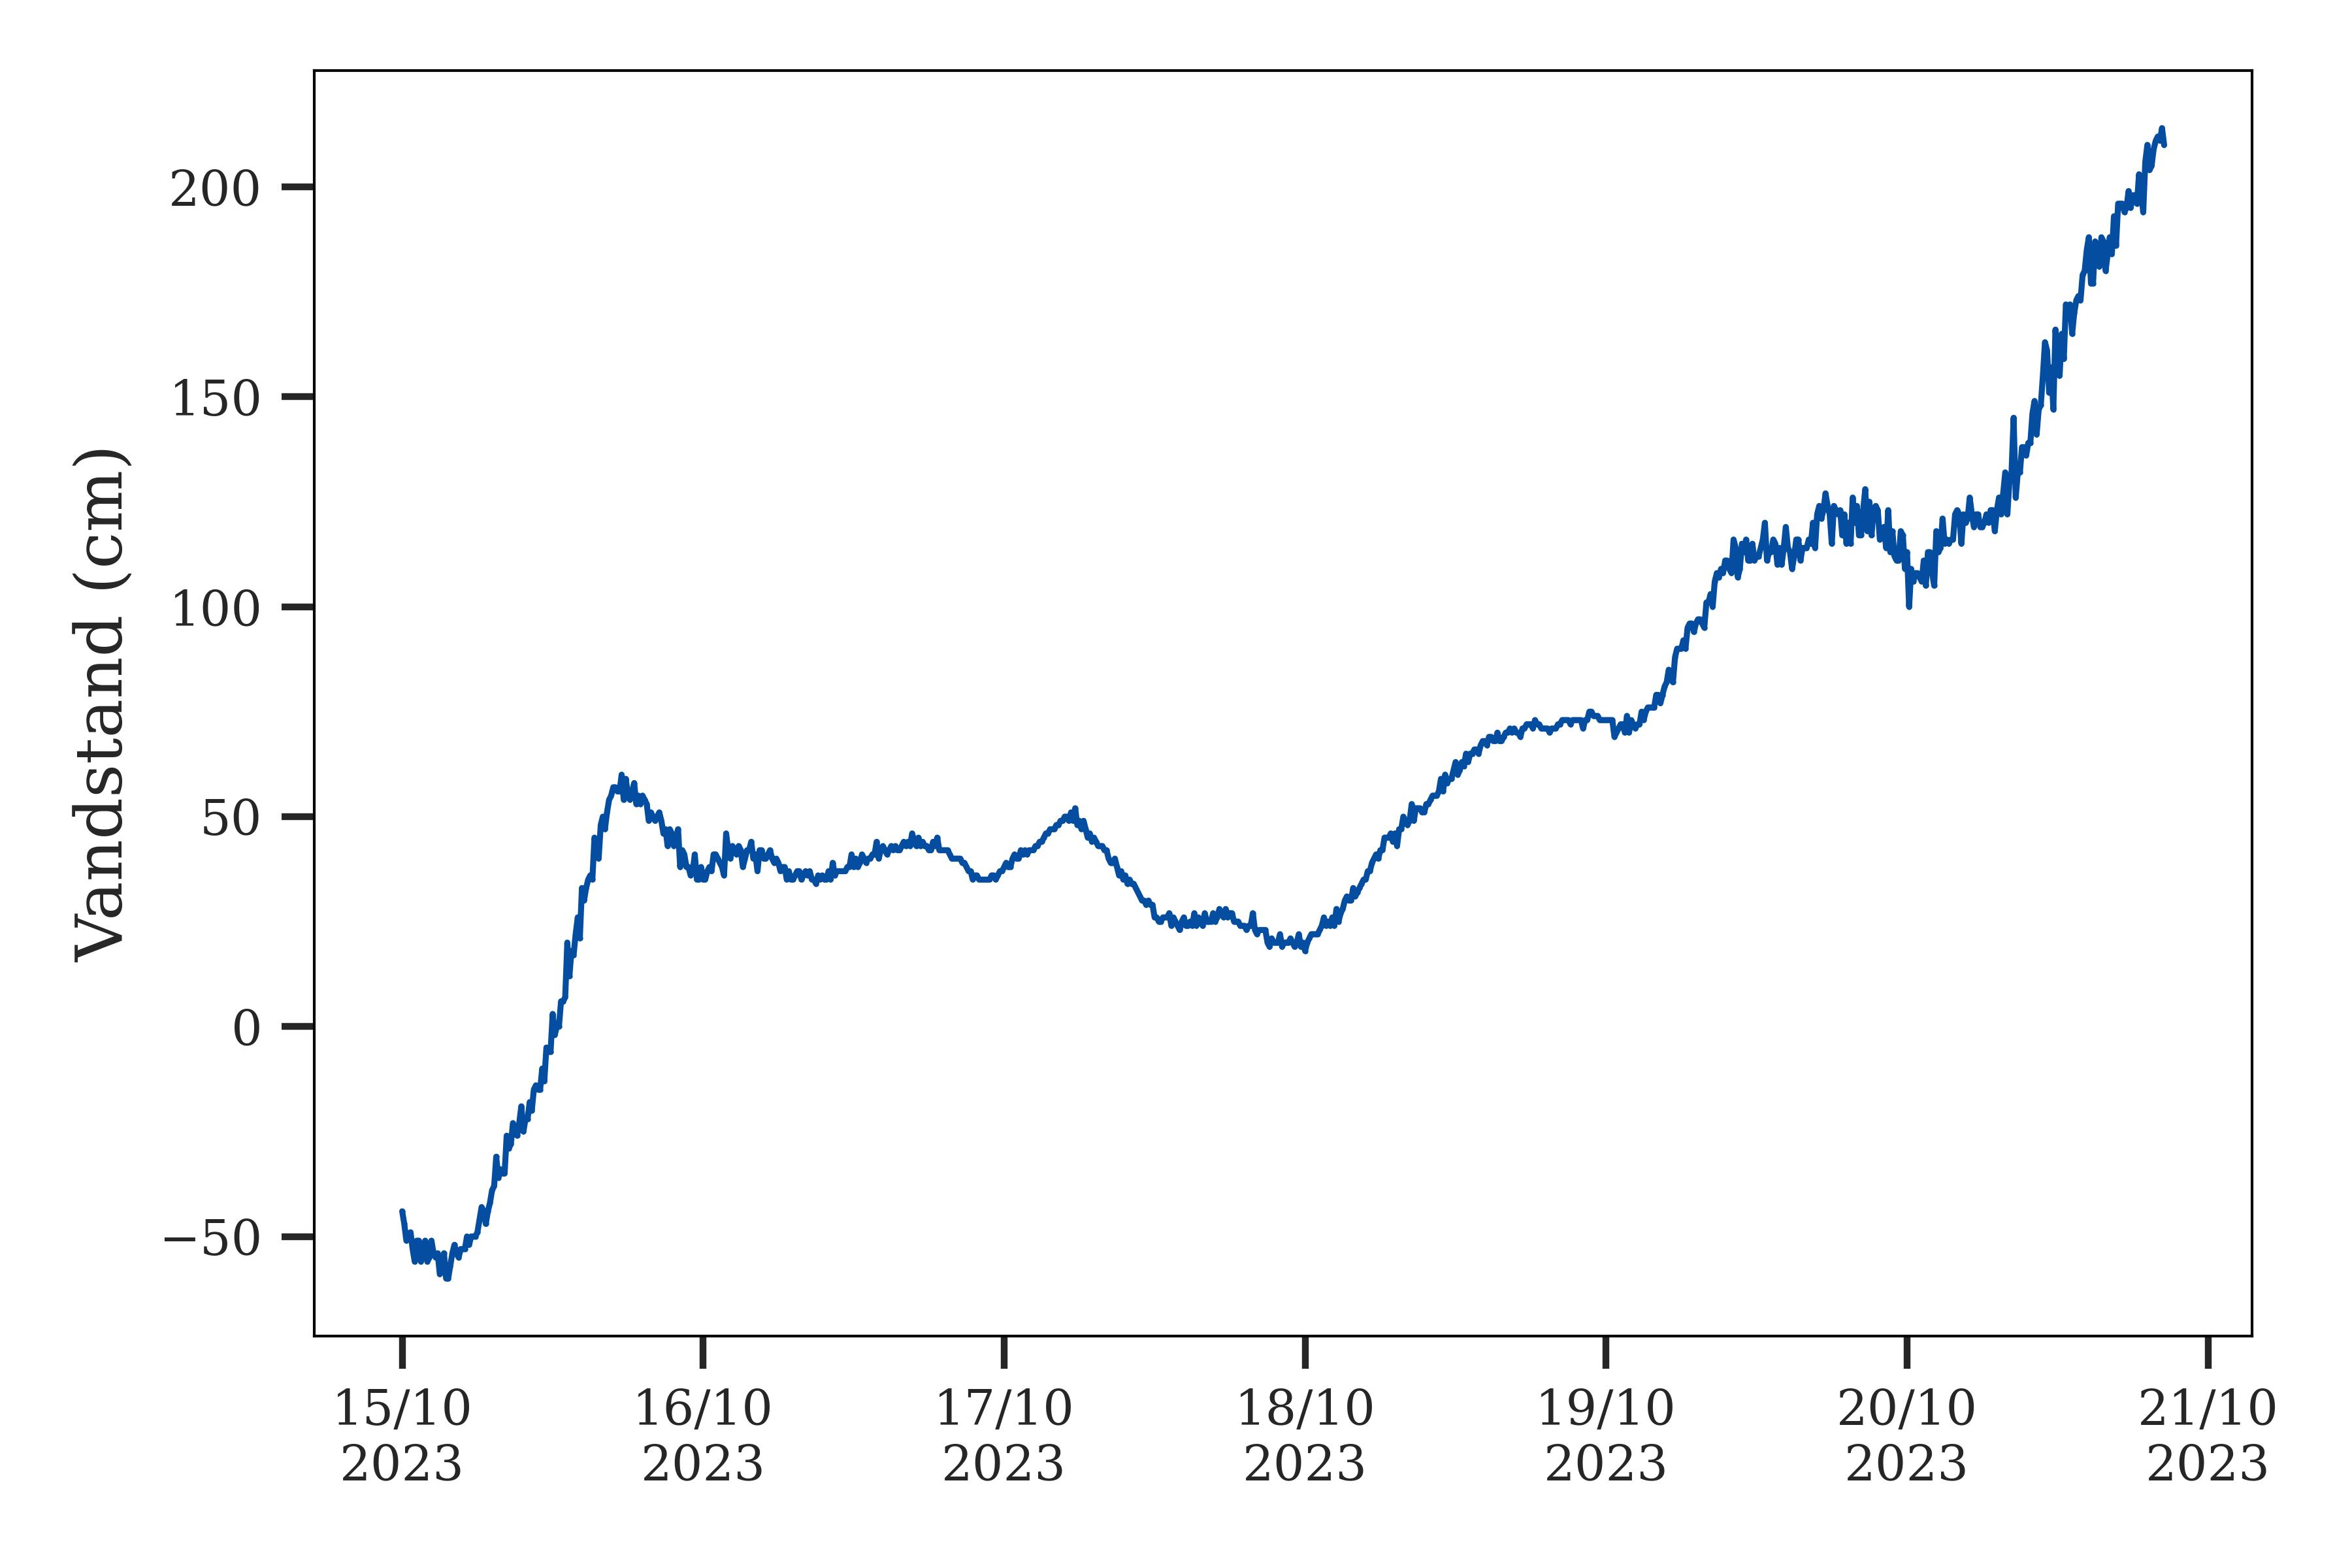
\includegraphics[width=1\textwidth]{images/studieområder/vandstands_grafer/vandstand_hesnaes_vandstandsplot.jpg}
        \caption{}
        \label{Subfig: Hesnæs vandstand}
    \end{subfigure}
    \hspace{0.2cm}
    \begin{subfigure}[b]{0.5\textwidth}
        \centering
        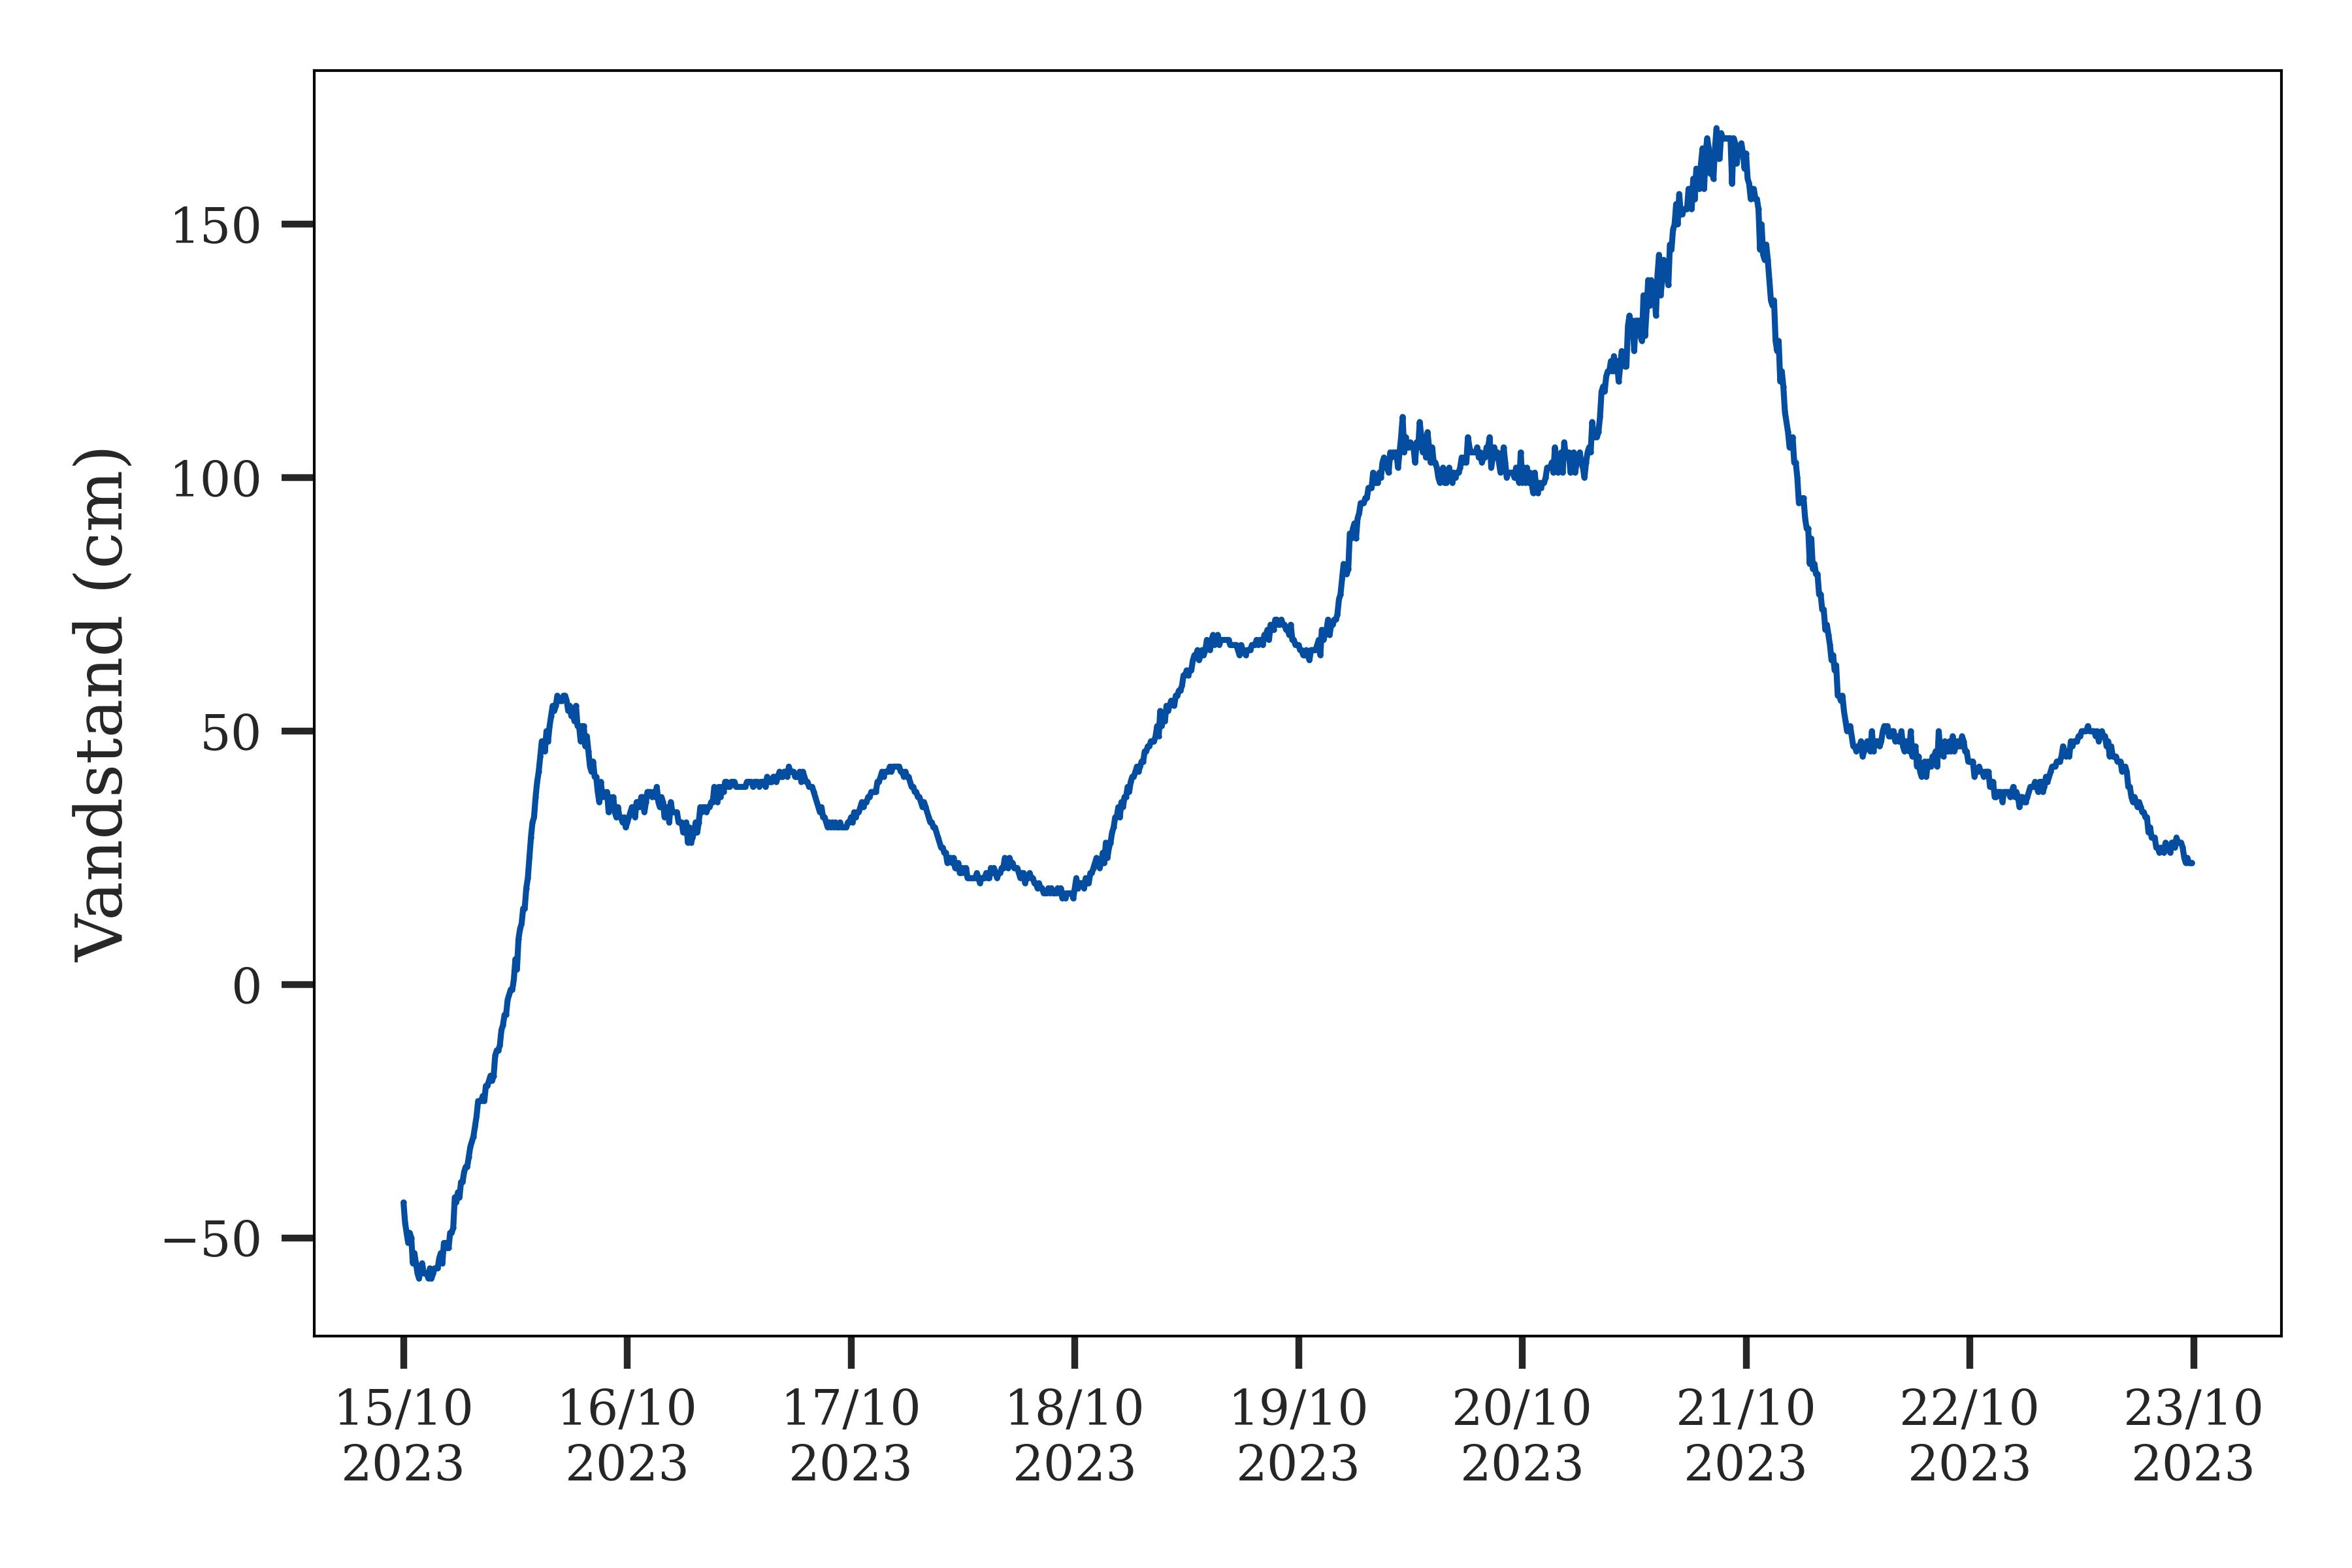
\includegraphics[width=1\textwidth]{images/studieområder/vandstands_grafer/vandstand_praestoe_roedvig_vandstandsplot.jpg}
        \caption{}
        \label{Subfig: Rødvig vandstand}
    \end{subfigure}
    \caption{Officiel målt vandstandsniveau i Aabenraa, Gedser Havn, Hesnæs og Rødvig fra den 15. til 23. oktober. \textbf{(a)} Vandstanden i Aabenraa fra 15. til 23. oktober 2023. \textbf{(b)} Vandstanden i Gedser Havn fra 15. til 23. oktober 2023. \textbf{(c)} Vandstanden i Hesnæs fra 15. til 21. oktober 2023. \textbf{(d)} Vandstanden i Rødvig fra 15. til 23. oktober 2023. Kilde: Data stammer fra DMI og DMIs Frie Data API-ressource.}
    \label{Figur: Vandstandsdata}
\end{figure}
{\large Hesnæs}\\
Hesnæs er et lille fiskerleje og landsby på det østlige Falster i Guldborgsund kommune. Hesnæs fungerer dagligt som en fiskeri- og lystbådehavn og er den eneste havn på Falsters østkyst. Hesnæs er beliggende inde mellem to skove: Corselitze skov mod nord og Bønnet skov mod syd, som begge går ud til skrånede klinter ud til Østersøen og danner et naturligt lavtliggende område ved landsbyen. \\
Hesnæs blev særdeles hårdt ramt af stormfloden, hvor der blev officielt målt 2,10 m vandstand over DVR90. Uofficielle målinger nåede op på 2,39 meter over DVR90, men vandstandsmåleren gik i stykker kort tid efter kl. 20:30 den 20. oktober (figur \ref{Subfig: Hesnæs vandstand}). Meget af Hesnæs havn blev svært beskadiget af stormfloden på grund af Hesnæs eksponering og større fristræk mod Østersøen. Især den ydre mole af havnen blev ødelagt af høje bølger og broerne i havnen blev skyllet på land. Lystbådehavnen er på nuværende tidspunkt stadig ude af drift og skaderne på havnens mole er stadig synlige.\\

{\large Præstø}\\
Præstø er en havneby og tidligere købstad i Vordingborg Kommune på Sjælland. Byen er beliggende i den sydlige del af Præstø Fjord, bag halvøen Feddet i bunden af Faxe Bugt. Tværs igennem byen løber Tubæk Å, et vandløb der løber fra tunneldalen Tubæk lidt syd for byen. Tubæk Å deler Præstø mellem et nordligt handelscentrum og et sydligt boligkvarter. Byen har en befolkningstal på ca. 4000 i 2025 \citep{danmarks_statistisk_mobile_nodate} og er kommunens andenstørste by.\\
Under stormfloden blev store dele af Præstøs nordlige handelscentrum oversvømmet, især efter sluseporten der bruges til at regulere vandniveauet i Tubæk Å, brød sammen \citep{uldall_sluseport_2023}. Der er ingen officielle målinger om vandstandshøjden i Præstø under stormfloden, da den nærmeste målestation er placeret længere opstrøms i Tubæk Å. \cite{cowi_praesto_2025} giver et skøn på at vandstanden var ca. 40 cm højere end i Rødvig Havn i Stevns Kommune ca. 25 km nordøst fra Præstø. Dette giver en vandstand på ca. 2 meter over DVR90 under stormfloden i Præstø (figur \ref{Subfig: Rødvig vandstand}).